\documentclass[tikz,border=3pt]{standalone}
\usepackage[T1]{fontenc}
\usepackage{times}
\usepackage{xcolor}
\usepackage{tikz}
\usetikzlibrary{arrows.meta,positioning}

\definecolor{huntrixblue}{HTML}{1F5A7A}
\definecolor{huntrixgold}{HTML}{D59B32}
\definecolor{huntrixgray}{HTML}{EEF2F4}
\newcommand{\labelzero}{\texttt{label=0}}
\newcommand{\labelone}{\texttt{label=1}}

\begin{document}
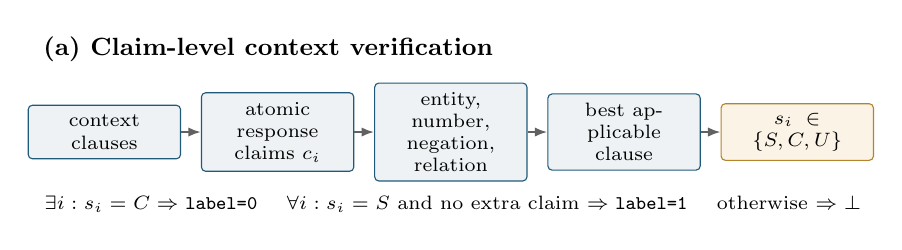
\begin{tikzpicture}[
  every node/.style={font=\scriptsize},
  box/.style={draw=huntrixblue, rounded corners=1.5pt, fill=huntrixgray,
              minimum height=6.8mm, align=center, text width=17mm},
  outcome/.style={draw=huntrixgold!85!black, rounded corners=1.5pt,
                  fill=huntrixgold!12, minimum height=6.8mm,
                  align=center, text width=17mm},
  arrow/.style={-{Latex[length=1.6mm]}, thick, draw=black!62}
]
\node[font=\small\bfseries, anchor=west] at (0,1.05) {(a) Claim-level context verification};
\node[box] (clauses) at (0.9,0) {context\\clauses};
\node[box] (claims) at (3.1,0) {atomic response\\claims $c_i$};
\node[box] (anchors) at (5.3,0) {entity, number,\\negation, relation};
\node[box] (align) at (7.5,0) {best applicable\\clause};
\node[outcome] (state) at (9.7,0) {$s_i\in\{S,C,U\}$};
\draw[arrow] (clauses) -- (claims);
\draw[arrow] (claims) -- (anchors);
\draw[arrow] (anchors) -- (align);
\draw[arrow] (align) -- (state);
\node[anchor=west, text width=104mm, align=center] at (0,-0.92)
  {$\exists i:s_i=C\Rightarrow\labelzero$ \quad
   $\forall i:s_i=S$ and no extra claim $\Rightarrow\labelone$ \quad
   otherwise $\Rightarrow\bot$};
\end{tikzpicture}
\end{document}
